% hand_built.tex

\marginnote{beginning of models/hand\_built.tex}

\subsection{Build an interesting grammar by hand}

We would like to demonstrate the expressiveness of grammatical curve
models. In particular, we would like to show that a hand-built grammar
can exhibit interesting variation, such as:
\begin{itemize}      
 \item articulating parts of an object (fingers on the hand)
 \item the presence or absence of a part (thumb on the hand)
 \item a choice between two different variations on a part (pants vs. skirt)
 \item shared parts that occur in different contexts (fingers on the hand)
\end{itemize}

\marginnote{Move this experiment to the section on building a grammar
  from a single curve?}

We have built three grammar by hand, by taking the following curves, and
specifying decompositions of them:

\begin{figure}
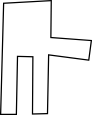
\includegraphics[width=\linewidth]{output/1.models/hand_built/hand_curve.png}
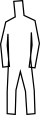
\includegraphics[width=\linewidth]{output/1.models/hand_built/romer_curve.png}
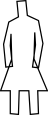
\includegraphics[width=\linewidth]{output/1.models/hand_built/romer_skirt.png}
\caption{The initial curves}
\end{figure}

\marginnote{Actually write out some of the rules of both grammars, and
  then use the nonterminal names in figure captions.}

Here are some samples from the three grammars:
\begin{figure}
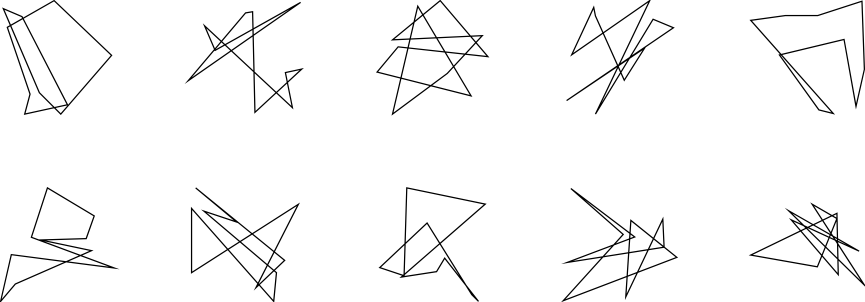
\includegraphics[width=\linewidth]{output/1.models/hand_built/romer/samples.png}
\end{figure}

\begin{figure}
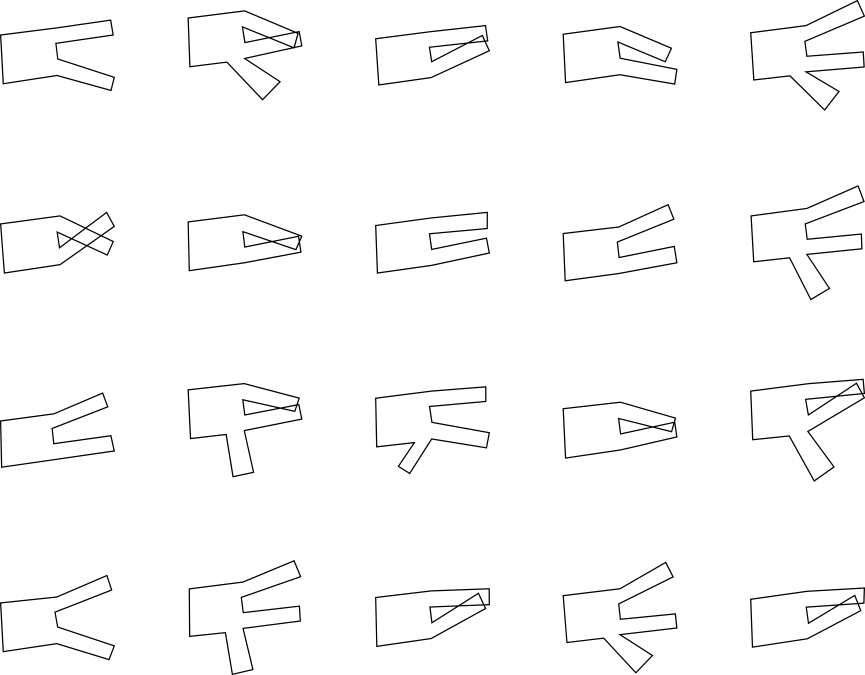
\includegraphics[width=\linewidth]{output/1.models/hand_built/hand/samples.png}
\end{figure}

\begin{figure}
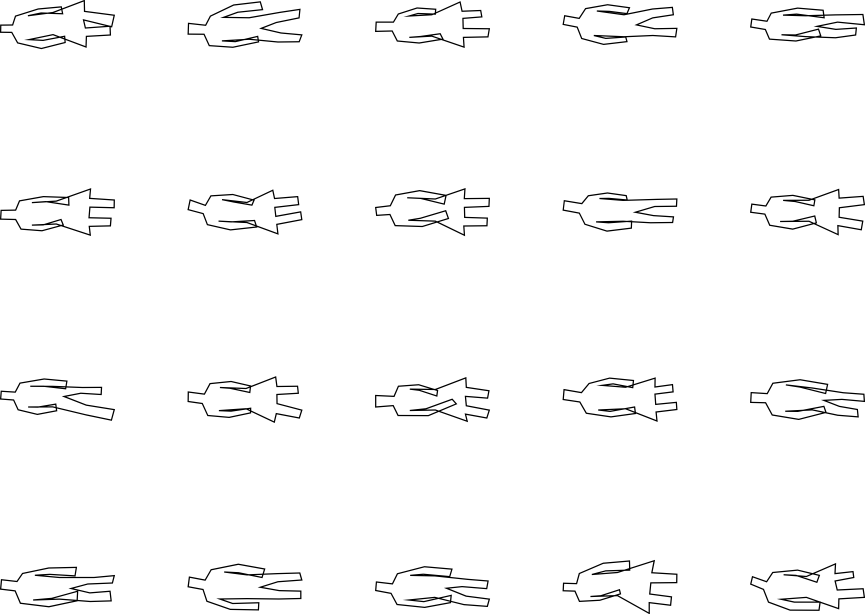
\includegraphics[width=\linewidth]{output/1.models/hand_built/romerchoice/samples.png}
\end{figure}

Here we draw some of the nonterminals of the grammar. Note that we are
not drawing actual samples, but rather the original subcurve that gave
rise to this nonterminal, with the midpoint perturbed according to the
midpoint distribution associated with the nonterminal's sole non-lexical
production.

\begin{figure}
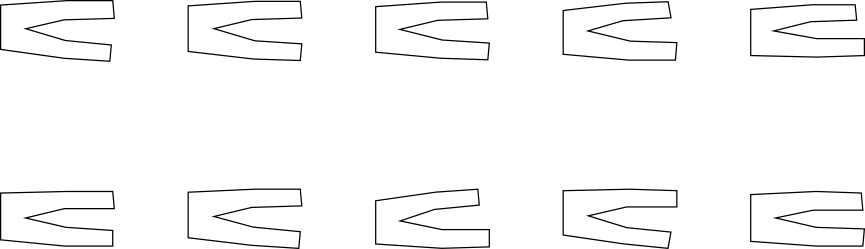
\includegraphics[width=\linewidth]{output/1.models/hand_built/romer/gram.0002.sample.png}
\end{figure}

\begin{figure}
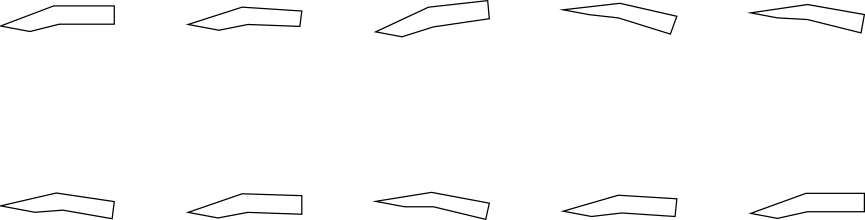
\includegraphics[width=\linewidth]{output/1.models/hand_built/romer/gram.0007.sample.png}
\end{figure}

\begin{figure}
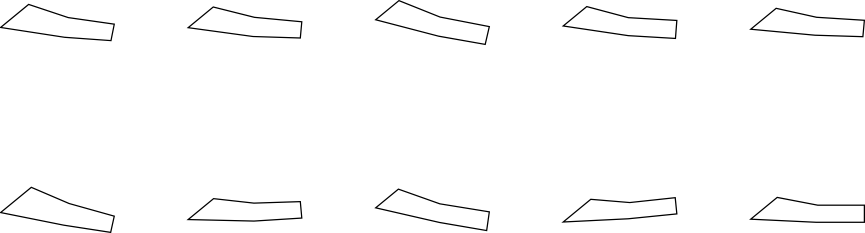
\includegraphics[width=\linewidth]{output/1.models/hand_built/romer/gram.0018.sample.png}
\end{figure}


\begin{figure}
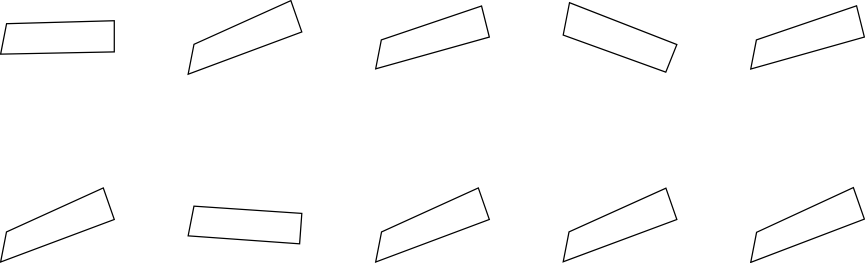
\includegraphics[width=\linewidth]{output/1.models/hand_built/hand/gram.0008.sample.png}
\caption{$X_{finger}$}
\end{figure}

\begin{figure}
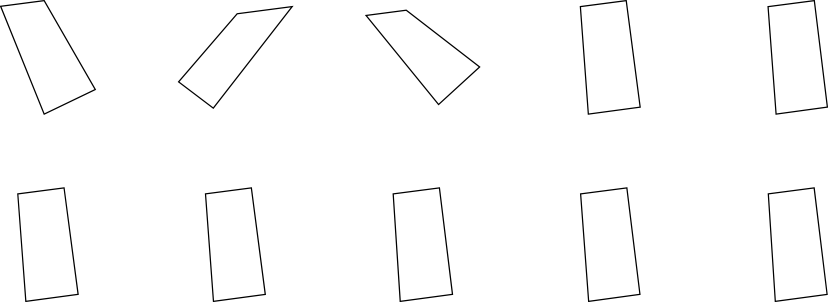
\includegraphics[width=\linewidth]{output/1.models/hand_built/hand/gram.0009.sample.png}
\caption{$X_{thumb}$}
\end{figure}

\FloatBarrier

\marginnote{end of models/hand\_built.tex}

